\documentclass[../AnalysisNoteJBuxton.tex]{subfiles}
\begin{document}

\subsection{Stavinsky Correlation Function Construction}
\label{StavCfConstruction}

The purpose of the Stavinsky method is to rid the correlation functions of the non-femtoscopic background.  More specifically, this method is intended to handle background contributions from elliptic flow, and other sources having reflection symmetry in the transverse plane.  With the Stavinsky method, mixed-event pairs are not used for the background; instead, same-event sudo-pairs, formed by rotating one particle in a real pair by 180$^\circ$ in the transverse plane, as used as a background.  This rotation rids the pairs of any femtoscopic correlation, while maintaining correlations due to elliptic flow (and other properly symmetric contributors).

The results of correctly implementing such a procedure are shown in Figure \ref{fig:AllStavCfs_Correct}.  The figure shows the Stavinsky method does a very good job of ridding the \LamKpm correlations of their non-femtoscopic backgrounds.  We also see the procedure does not work as well on the \LamKs system.


\begin{figure}[h!]
  \centering
  %%----start of first subfigure---  
  \subfloat[\LamKchP (left) and \ALamKchM (right).  Fully correct Stavinsky shown as open symbols.]{
    \label{fig:AllStavCfs_Correct:a}
    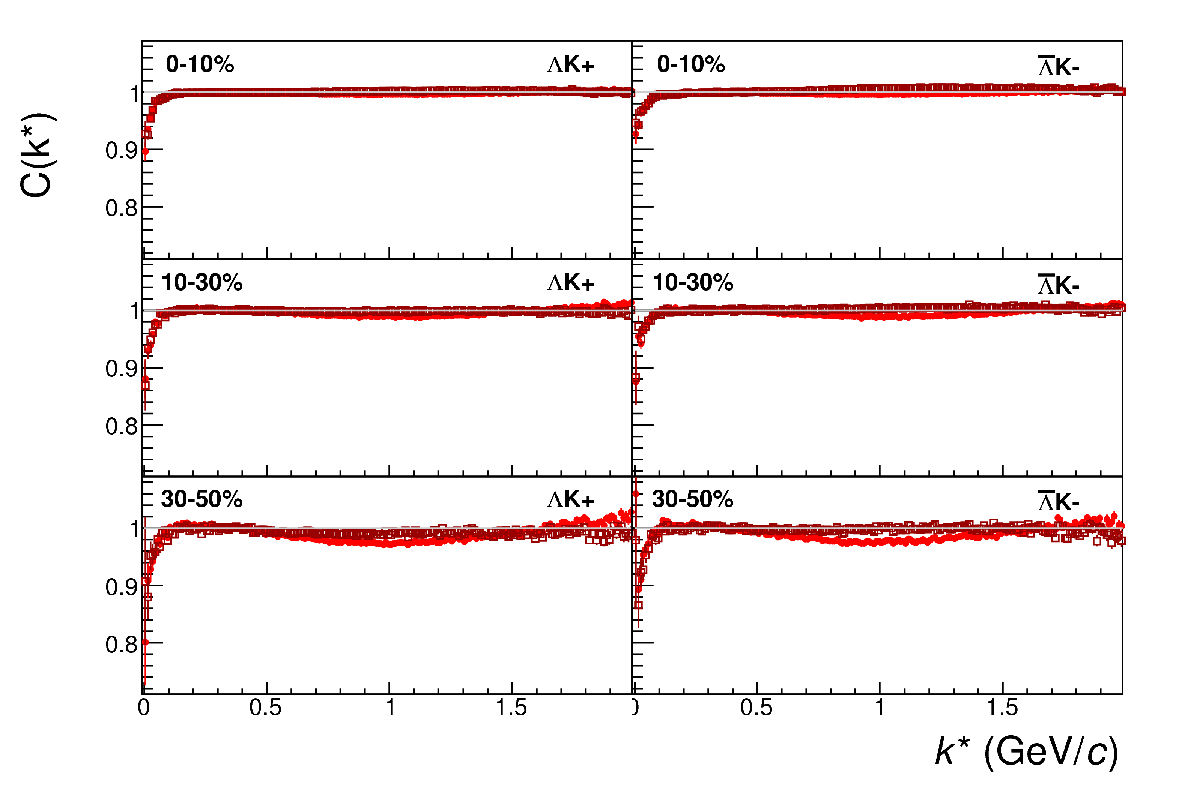
\includegraphics[width=0.49\textwidth]{4_CorrelationFunctions/Figures/WithAdditionalPairCut_20180505/canKStarCfsLamKchPwConj_20180505vs20180505StavCf.pdf}}
  %%----start of second subfigure---
  \subfloat[\LamKchM (left) and \ALamKchP (right).  Fully correct Stavinsky shown as open symbols.]{
    \label{fig:AllStavCfs_Correct:b}
    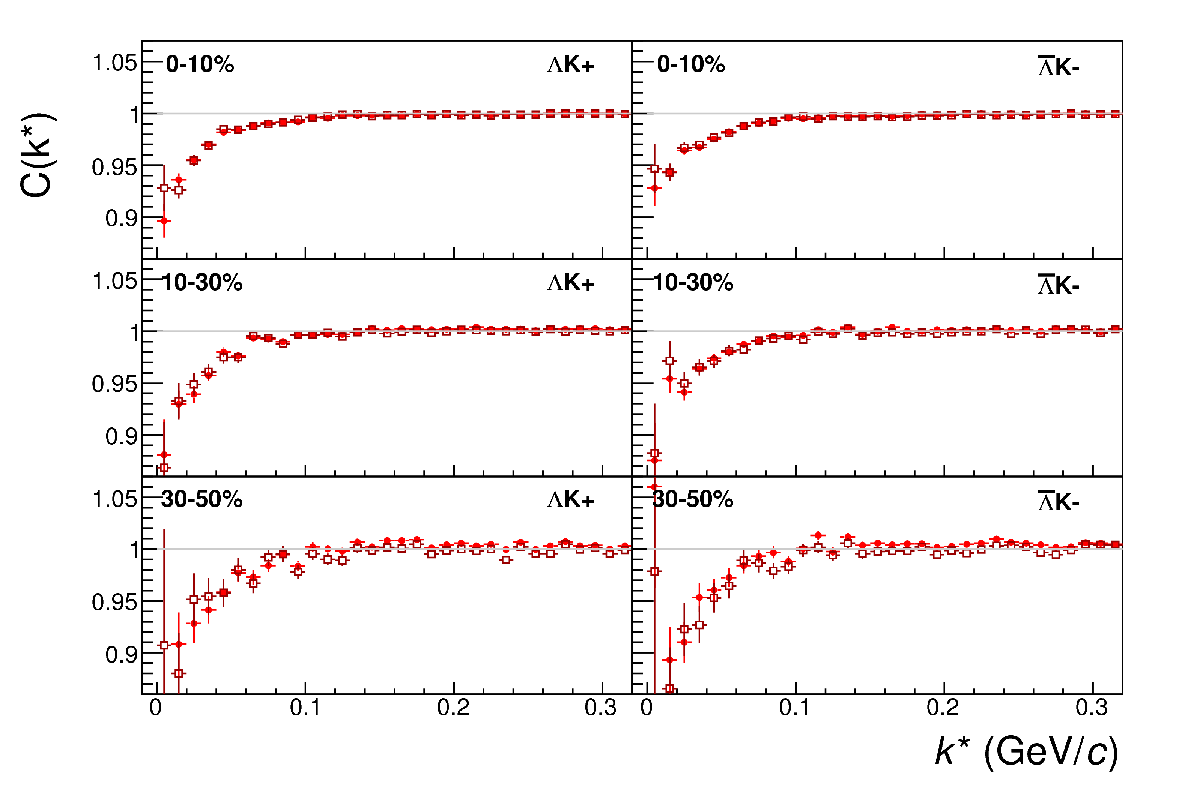
\includegraphics[width=0.49\textwidth]{4_CorrelationFunctions/Figures/WithAdditionalPairCut_20180505/canKStarCfsZoomLamKchPwConj_20180505vs20180505StavCf.pdf}}
  \\    
  
  %%----start of third subfigure---  
  \subfloat[\LamKchP (left) and \ALamKchM (right).  Fully correct Stavinsky shown as open symbols.]{
    \label{fig:AllStavCfs_Correct:c}
    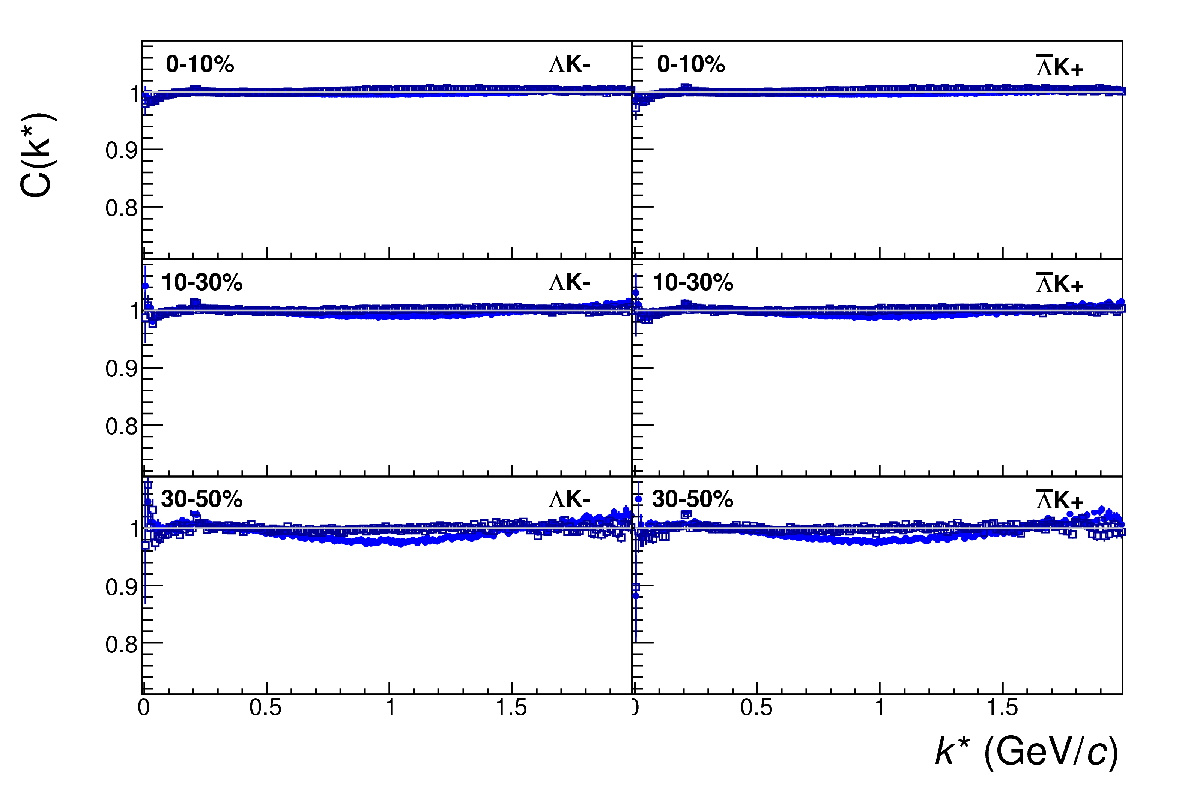
\includegraphics[width=0.49\textwidth]{4_CorrelationFunctions/Figures/WithAdditionalPairCut_20180505/canKStarCfsLamKchMwConj_20180505vs20180505StavCf.pdf}}
  %%----start of fourth subfigure---
  \subfloat[\LamKchM (left) and \ALamKchP (right).  Fully correct Stavinsky shown as open symbols.]{
    \label{fig:AllStavCfs_Correct:d}
    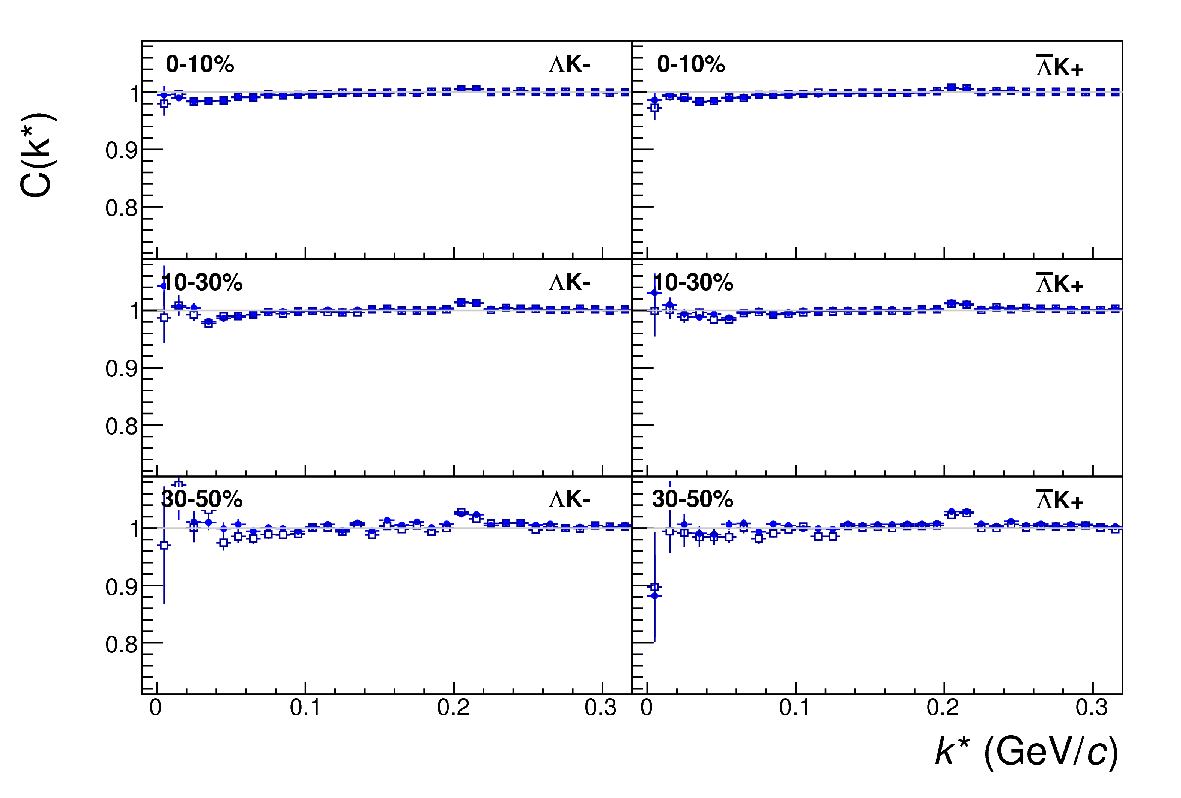
\includegraphics[width=0.49\textwidth]{4_CorrelationFunctions/Figures/WithAdditionalPairCut_20180505/canKStarCfsZoomLamKchMwConj_20180505vs20180505StavCf.pdf}}
  \\    
    
  %%----start of fifth subfigure---  
  \subfloat[\LamKchP (left) and \ALamKchM (right).  Fully correct Stavinsky shown as open symbols.]{
    \label{fig:AllStavCfs_Correct:e}
    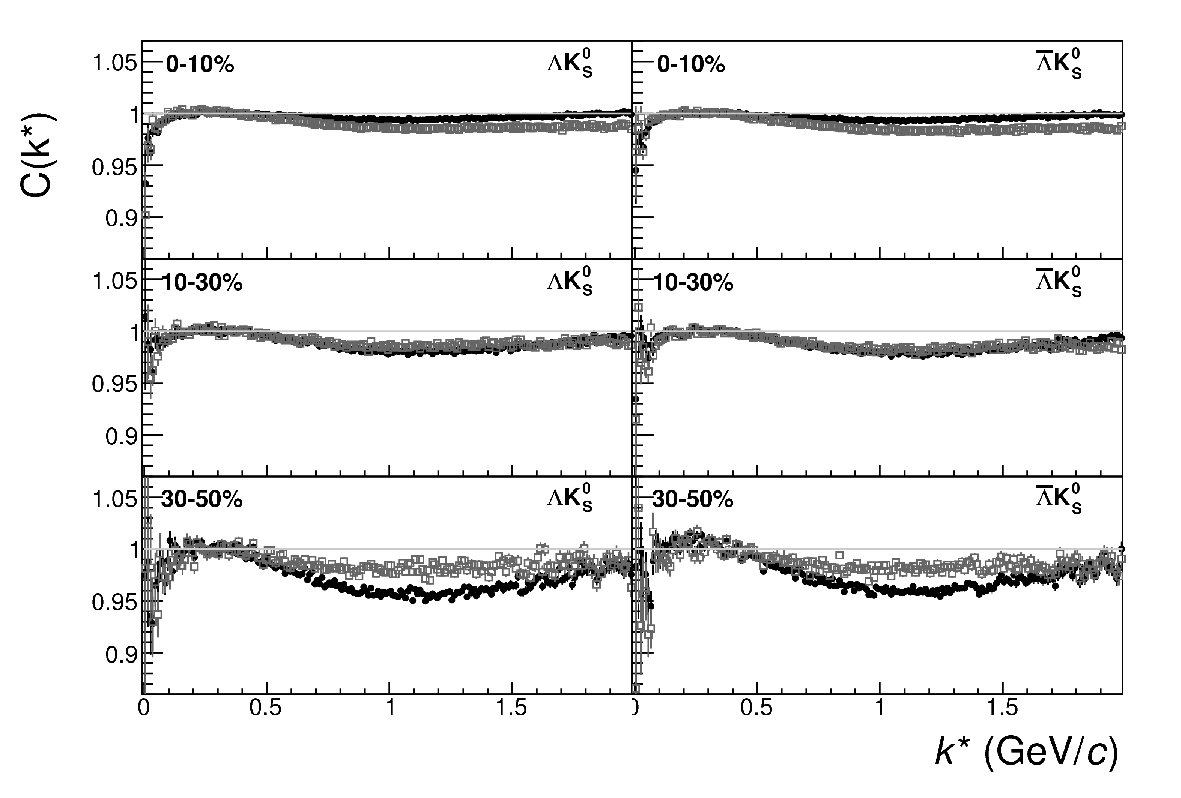
\includegraphics[width=0.49\textwidth]{4_CorrelationFunctions/Figures/WithAdditionalPairCut_20180505/canKStarCfsLamK0wConj_20180505vs20180505StavCf.pdf}}
  %%----start of sixth subfigure---
  \subfloat[\LamKchM (left) and \ALamKchP (right).  Fully correct Stavinsky shown as open symbols.]{
    \label{fig:AllStavCfs_Correct:f}
    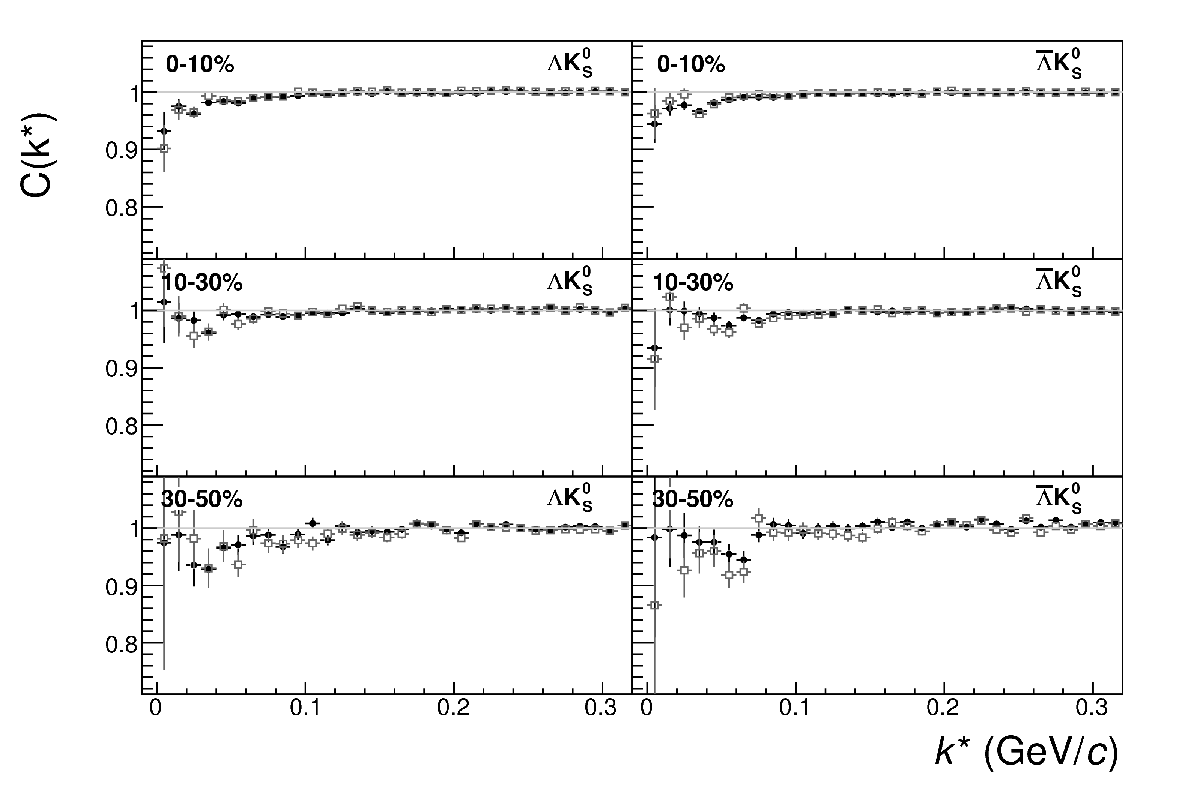
\includegraphics[width=0.49\textwidth]{4_CorrelationFunctions/Figures/WithAdditionalPairCut_20180505/canKStarCfsZoomLamK0wConj_20180505vs20180505StavCf.pdf}}
  \\         
    
  %%----overall caption----
  \caption[\LamK Stavinsky Correlation Functions (Correct)]{\LamK and \ALamAK correlation functions built using the fully correct Stavinsky method for 0-10\%, 10-30\%, and 30-50\% centralities.  In the full correct method, the pseudo-pairs (same-event pairs with one particle rotated by 180$^\circ$ in the transverse plane) are also run through the pair cuts used in the analysis.  Closed symbols represent correlations built using the normal mixed-event background, while open symbols represent correlations formed using the Stavinsky same-event pseudo-pairs as a background.  Figures in the right column are zoomed-in versions of figures in the left column.}
  \label{fig:AllStavCfs_Correct}
\end{figure}




Now, one must be somewhat careful when applying this Stavinsky method.  We found that, in order to obtain correct results, we had to run our pseudo-pairs through the same pair cuts used in our analyses.  In an ideal world, our pair cut would only remove truly bad pairs results from splitting, merging, etc.  In the real world, the pair cut always throws out some of the good with the bad.  For the pseudo-pairs to form a reliable background, they too must experience the pair cut, and the loss of "good" pairs.  We found this issue affected mainly our \LamKchP \& \ALamKchM analysis, as can be seen in Figure \ref{fig:AllStavCfs_Incorrect}, which shows an incorrect implementation of the Stavinsky method lacking the additional pair cut on the pseudo-pairs.






\begin{figure}[h!]
  \centering
  %%----start of first subfigure---  
  \subfloat[\LamKchP (left) and \ALamKchM (right).  Incorrect Stavinsky shown as open symbols.]{
    \label{fig:AllStavCfs_Incorrect:a}
    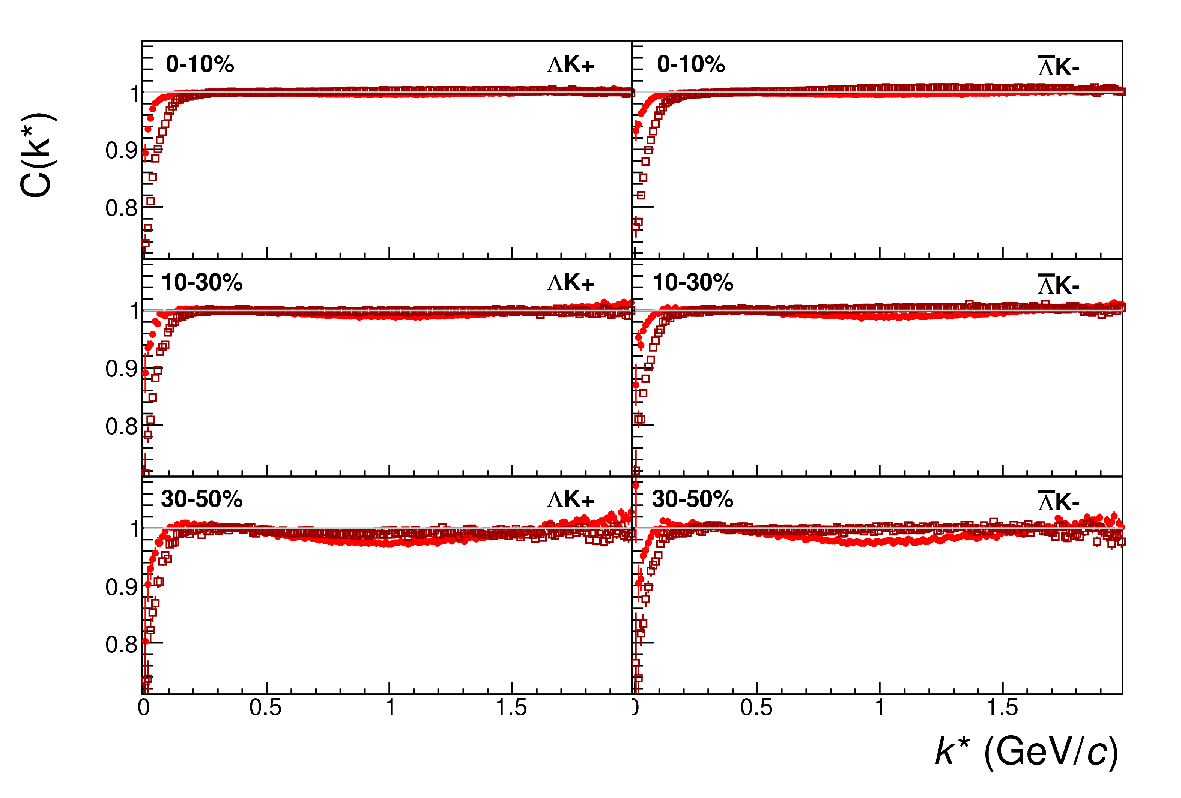
\includegraphics[width=0.49\textwidth]{4_CorrelationFunctions/Figures/WithoutAdditionalPairCut_20180416/canKStarCfsLamKchPwConj_20180416vs20180416StavCf.pdf}}
  %%----start of second subfigure---
  \subfloat[\LamKchM (left) and \ALamKchP (right).  Incorrect Stavinsky shown as open symbols.]{
    \label{fig:AllStavCfs_Incorrect:b}
    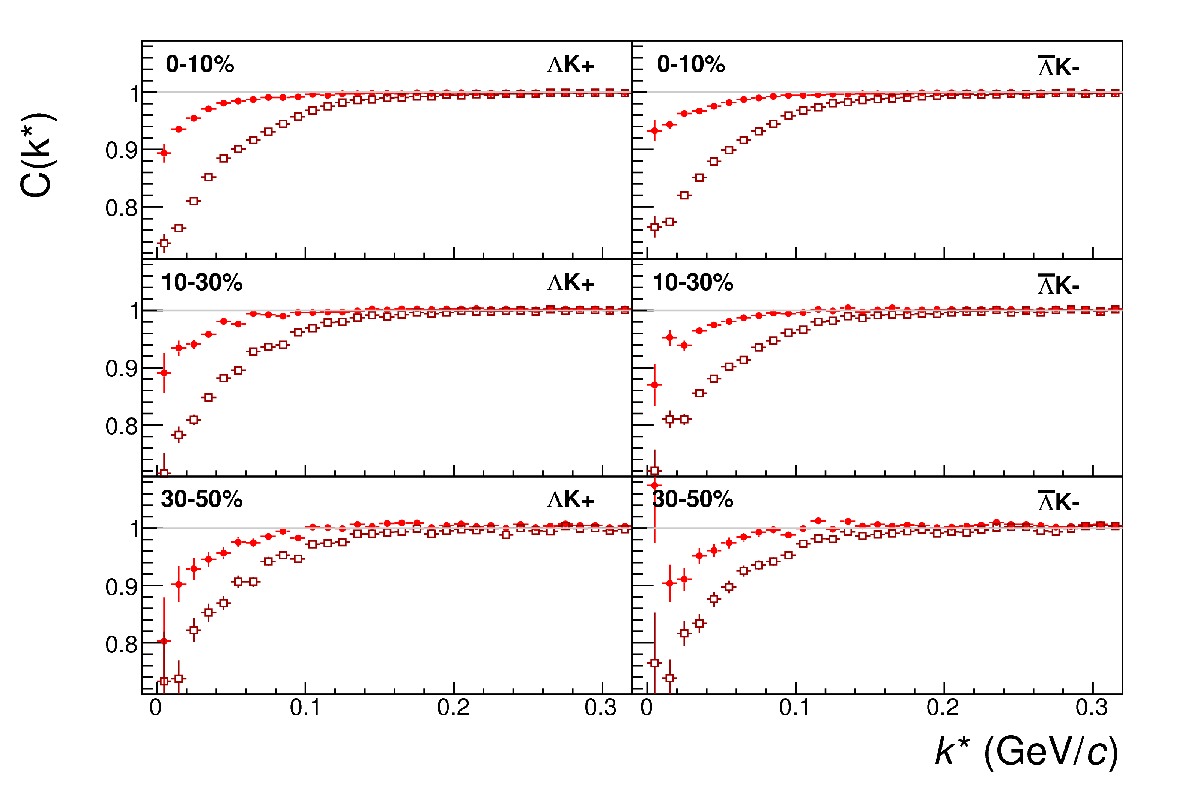
\includegraphics[width=0.49\textwidth]{4_CorrelationFunctions/Figures/WithoutAdditionalPairCut_20180416/canKStarCfsZoomLamKchPwConj_20180416vs20180416StavCf.pdf}}
  \\    
  
  %%----start of third subfigure---  
  \subfloat[\LamKchP (left) and \ALamKchM (right).  Incorrect Stavinsky shown as open symbols.]{
    \label{fig:AllStavCfs_Incorrect:c}
    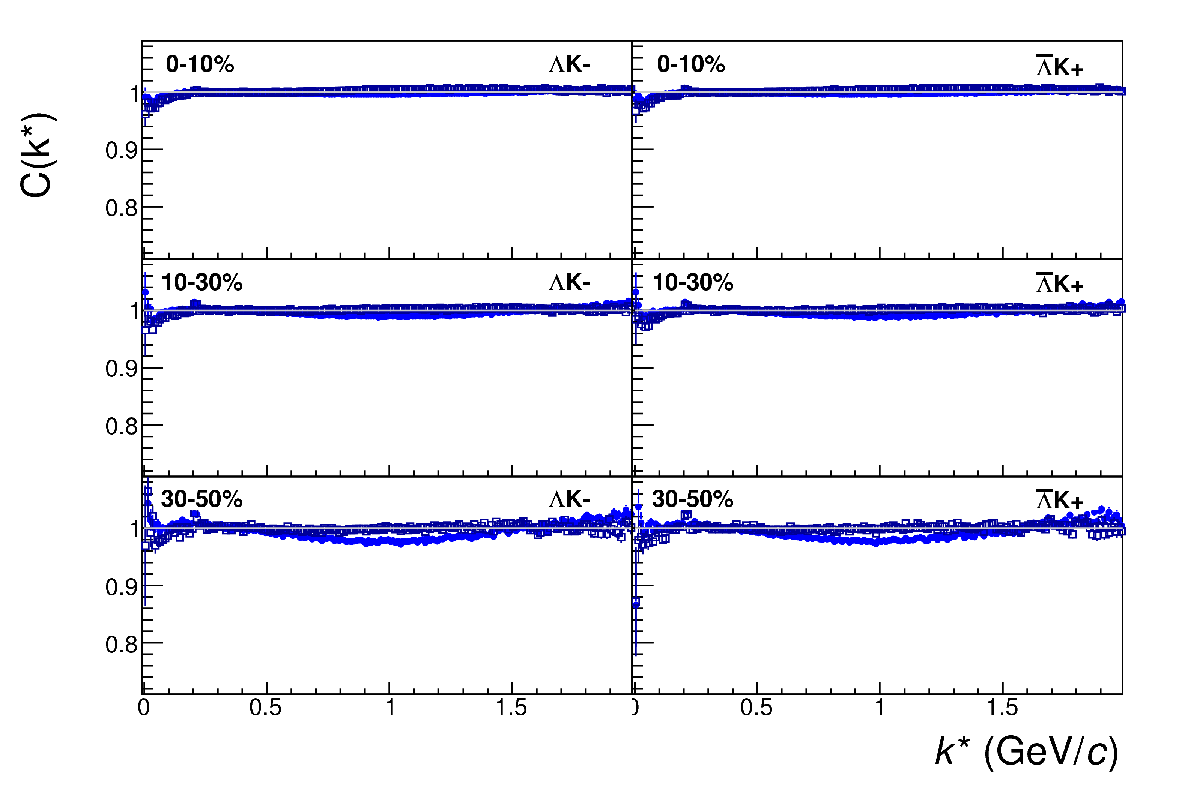
\includegraphics[width=0.49\textwidth]{4_CorrelationFunctions/Figures/WithoutAdditionalPairCut_20180416/canKStarCfsLamKchMwConj_20180416vs20180416StavCf.pdf}}
  %%----start of fourth subfigure---
  \subfloat[\LamKchM (left) and \ALamKchP (right).  Incorrect Stavinsky shown as open symbols.]{
    \label{fig:AllStavCfs_Incorrect:d}
    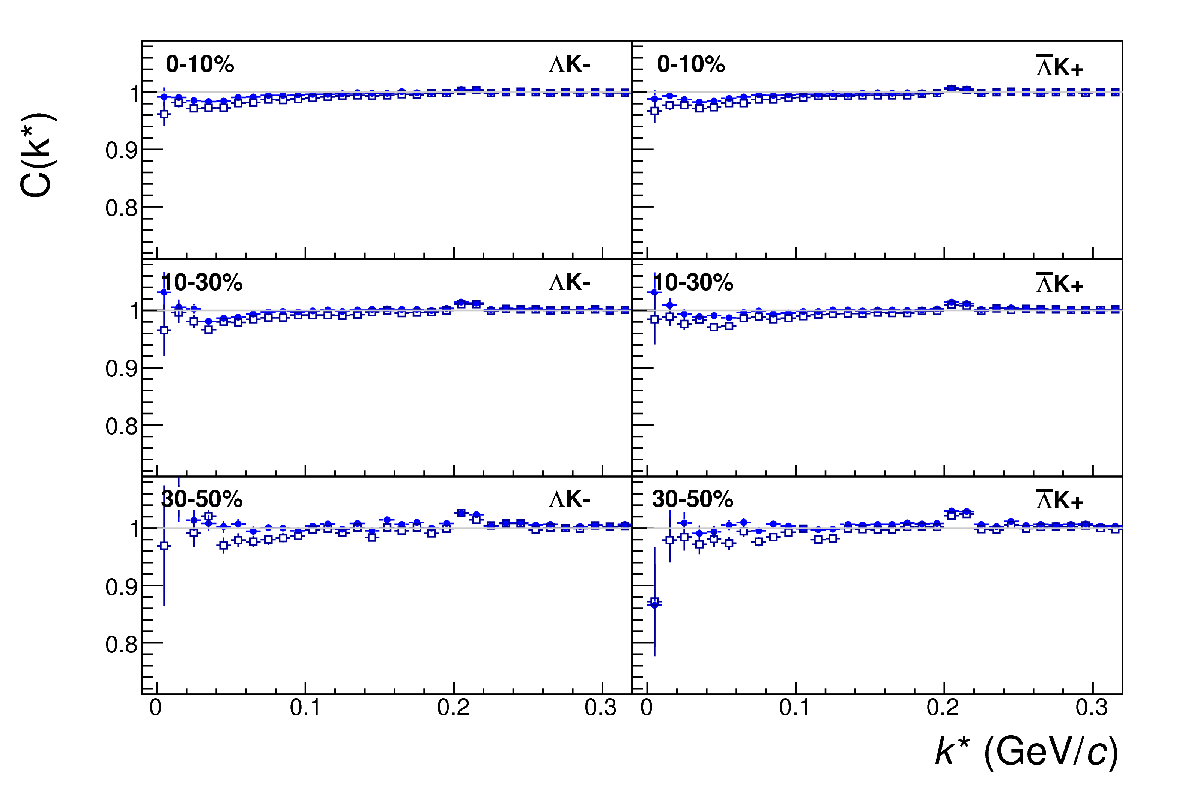
\includegraphics[width=0.49\textwidth]{4_CorrelationFunctions/Figures/WithoutAdditionalPairCut_20180416/canKStarCfsZoomLamKchMwConj_20180416vs20180416StavCf.pdf}}
  \\    
    
  %%----start of fifth subfigure---  
  \subfloat[\LamKchP (left) and \ALamKchM (right).  Incorrect Stavinsky shown as open symbols.]{
    \label{fig:AllStavCfs_Incorrect:e}
    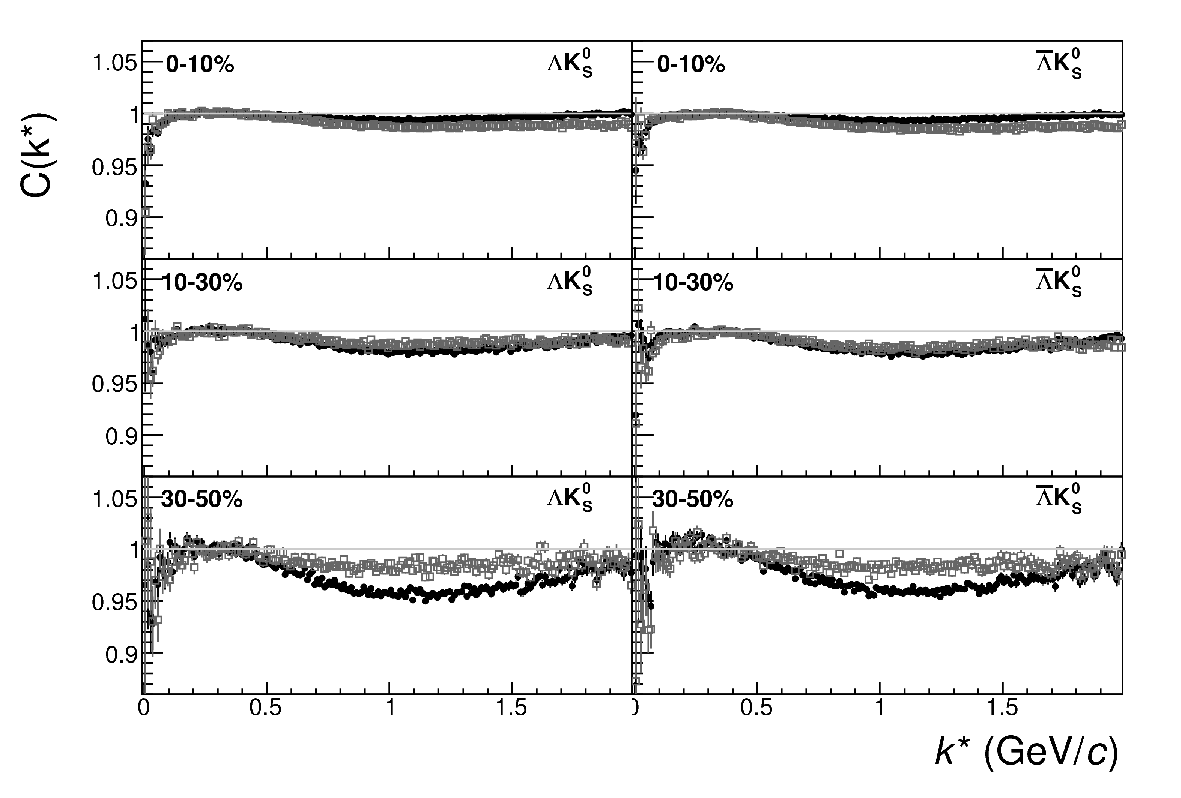
\includegraphics[width=0.49\textwidth]{4_CorrelationFunctions/Figures/WithoutAdditionalPairCut_20180416/canKStarCfsLamK0wConj_20180416vs20180416StavCf.pdf}}
  %%----start of sixth subfigure---
  \subfloat[\LamKchM (left) and \ALamKchP (right).  Incorrect Stavinsky shown as open symbols.]{
    \label{fig:AllStavCfs_Incorrect:f}
    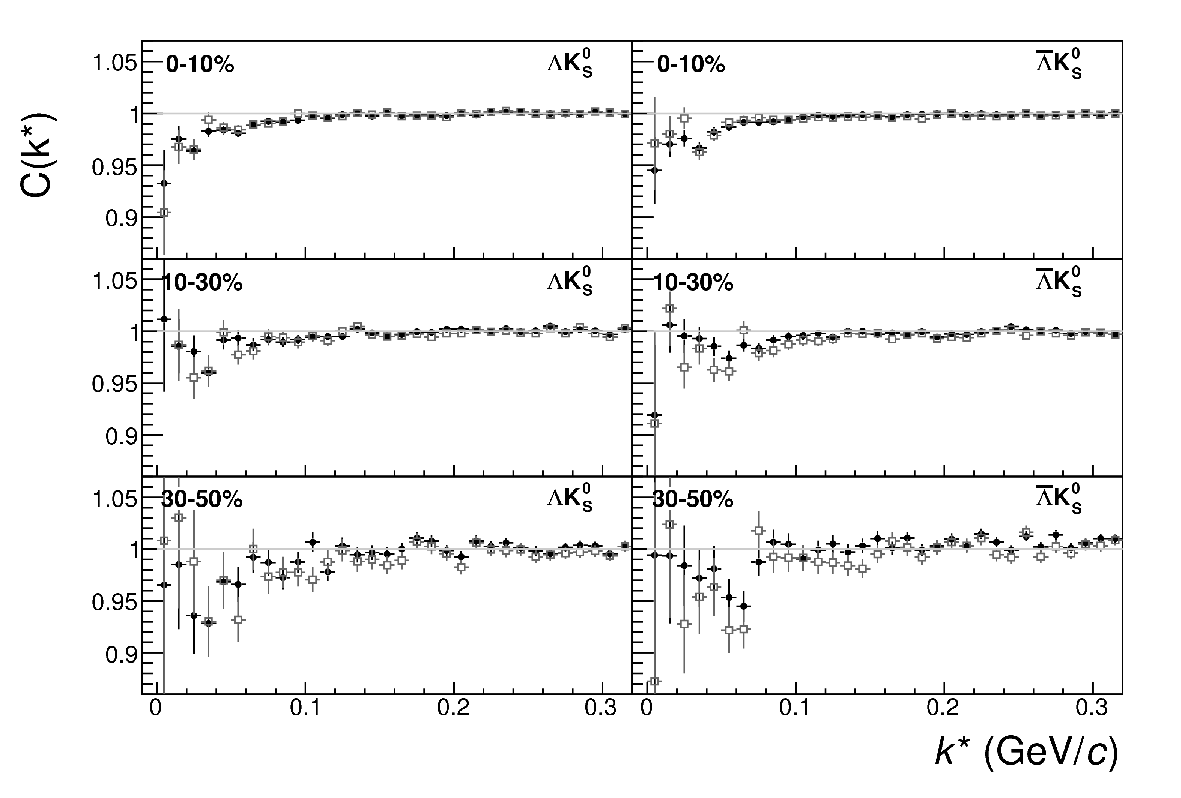
\includegraphics[width=0.49\textwidth]{4_CorrelationFunctions/Figures/WithoutAdditionalPairCut_20180416/canKStarCfsZoomLamK0wConj_20180416vs20180416StavCf.pdf}}
  \\         
    
  %%----overall caption----
  \caption[\LamK Stavinsky Correlation Functions (Incorrect)]{\LamK and \ALamAK correlation functions built using the incorrect Stavinsky method for 0-10\%, 10-30\%, and 30-50\% centralities.  In the incorrect method, the pseudo-pairs (same-event pairs with one particle rotated by 180$^\circ$ in the transverse plane) are not run through the pair cuts used in the analysis.  Closed symbols represent correlations built using the normal mixed-event background, while open symbols represent correlations formed using the Stavinsky same-event pseudo-pairs as a background.  Figures in the right column are zoomed-in versions of figures in the left column.}
  \label{fig:AllStavCfs_Incorrect}
\end{figure}




\begin{figure}[h!]
  \centering
  %%----start of first subfigure---  
  \subfloat[\LamKchP (left) and \ALamKchM (right).  Incorrect Stavinsky shown as open symbols.]{
    \label{fig:AllStavCfs_CorrectAndIncorrect:a}
    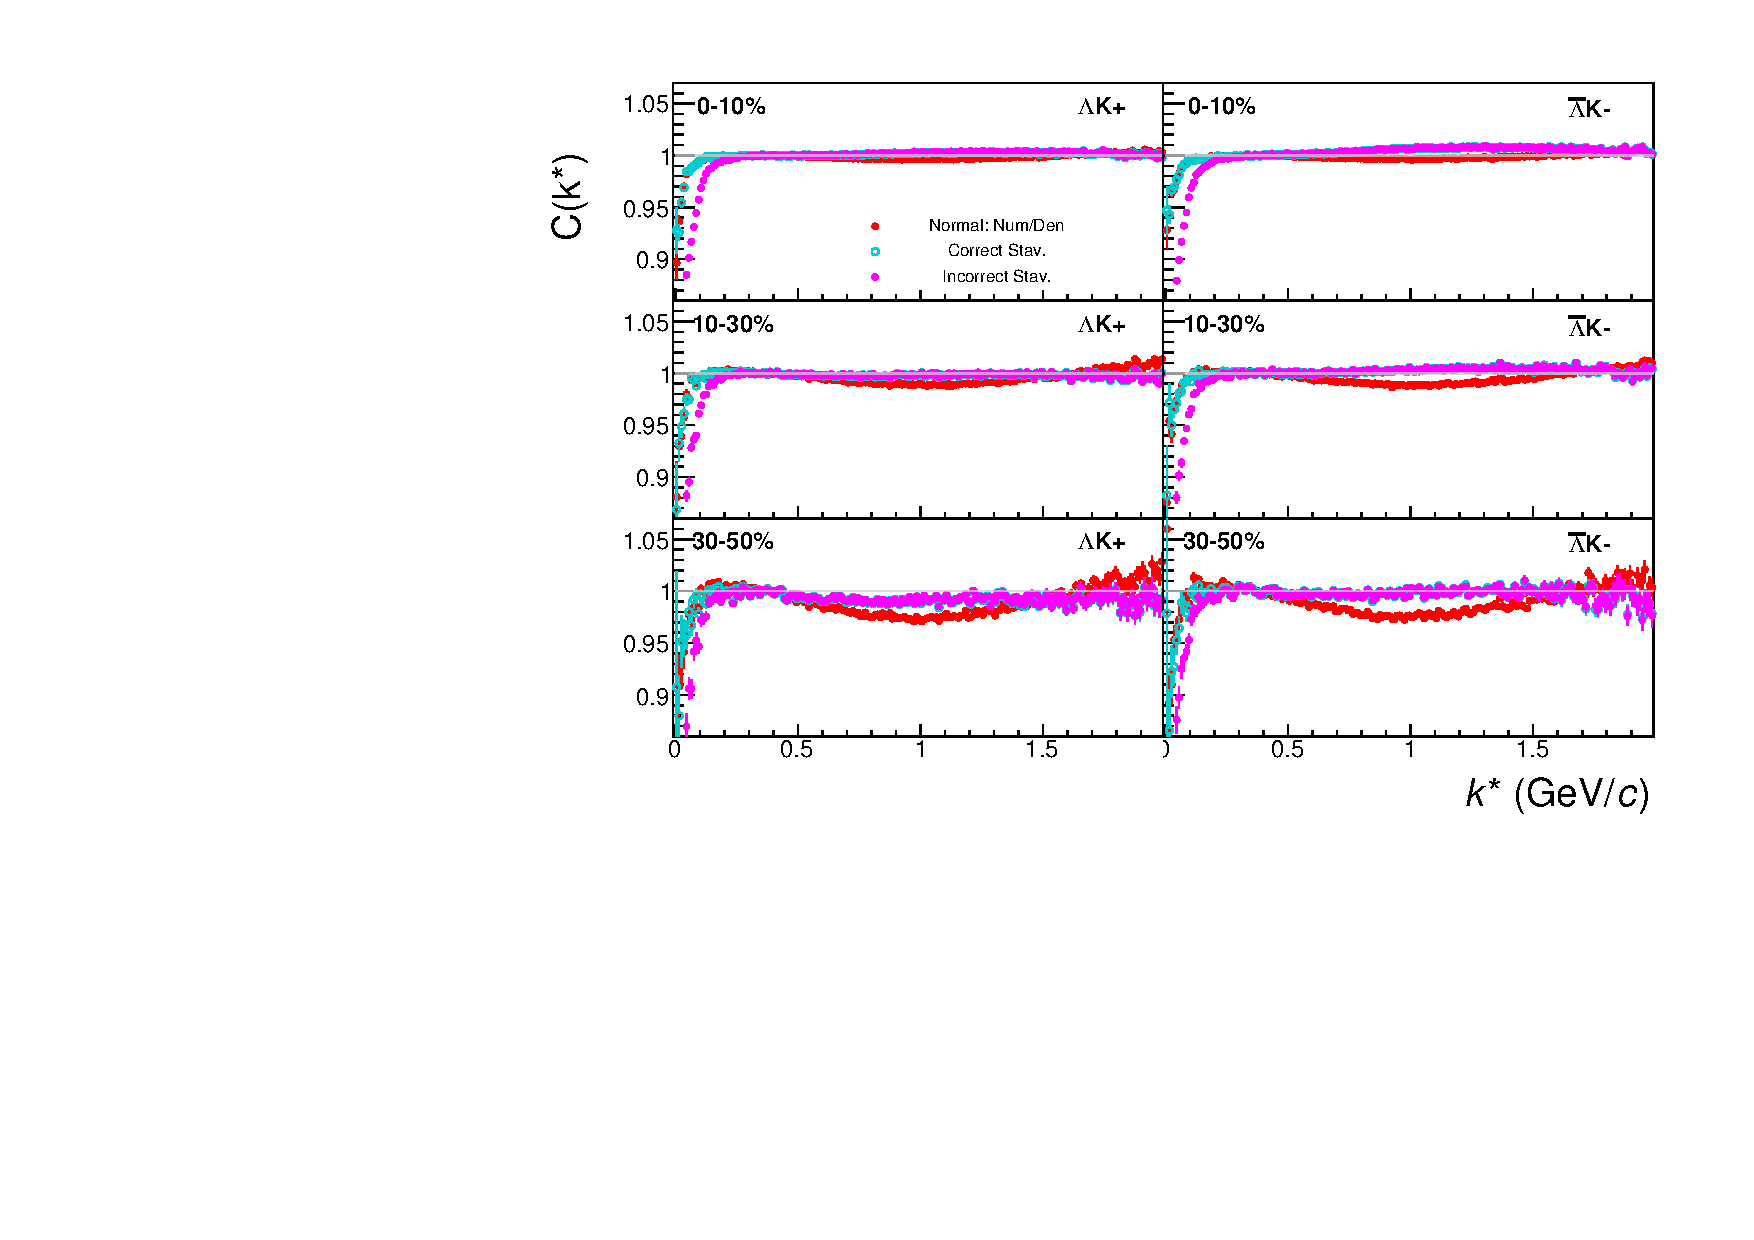
\includegraphics[width=0.49\textwidth]{4_CorrelationFunctions/Figures/AllThreeTogether/canKStarCfsLamKchPwConj_20180505vs20180505StavCfvs20180416StavCf.pdf}}
  %%----start of second subfigure---
  \subfloat[\LamKchM (left) and \ALamKchP (right).  Incorrect Stavinsky shown as open symbols.]{
    \label{fig:AllStavCfs_CorrectAndIncorrect:b}
    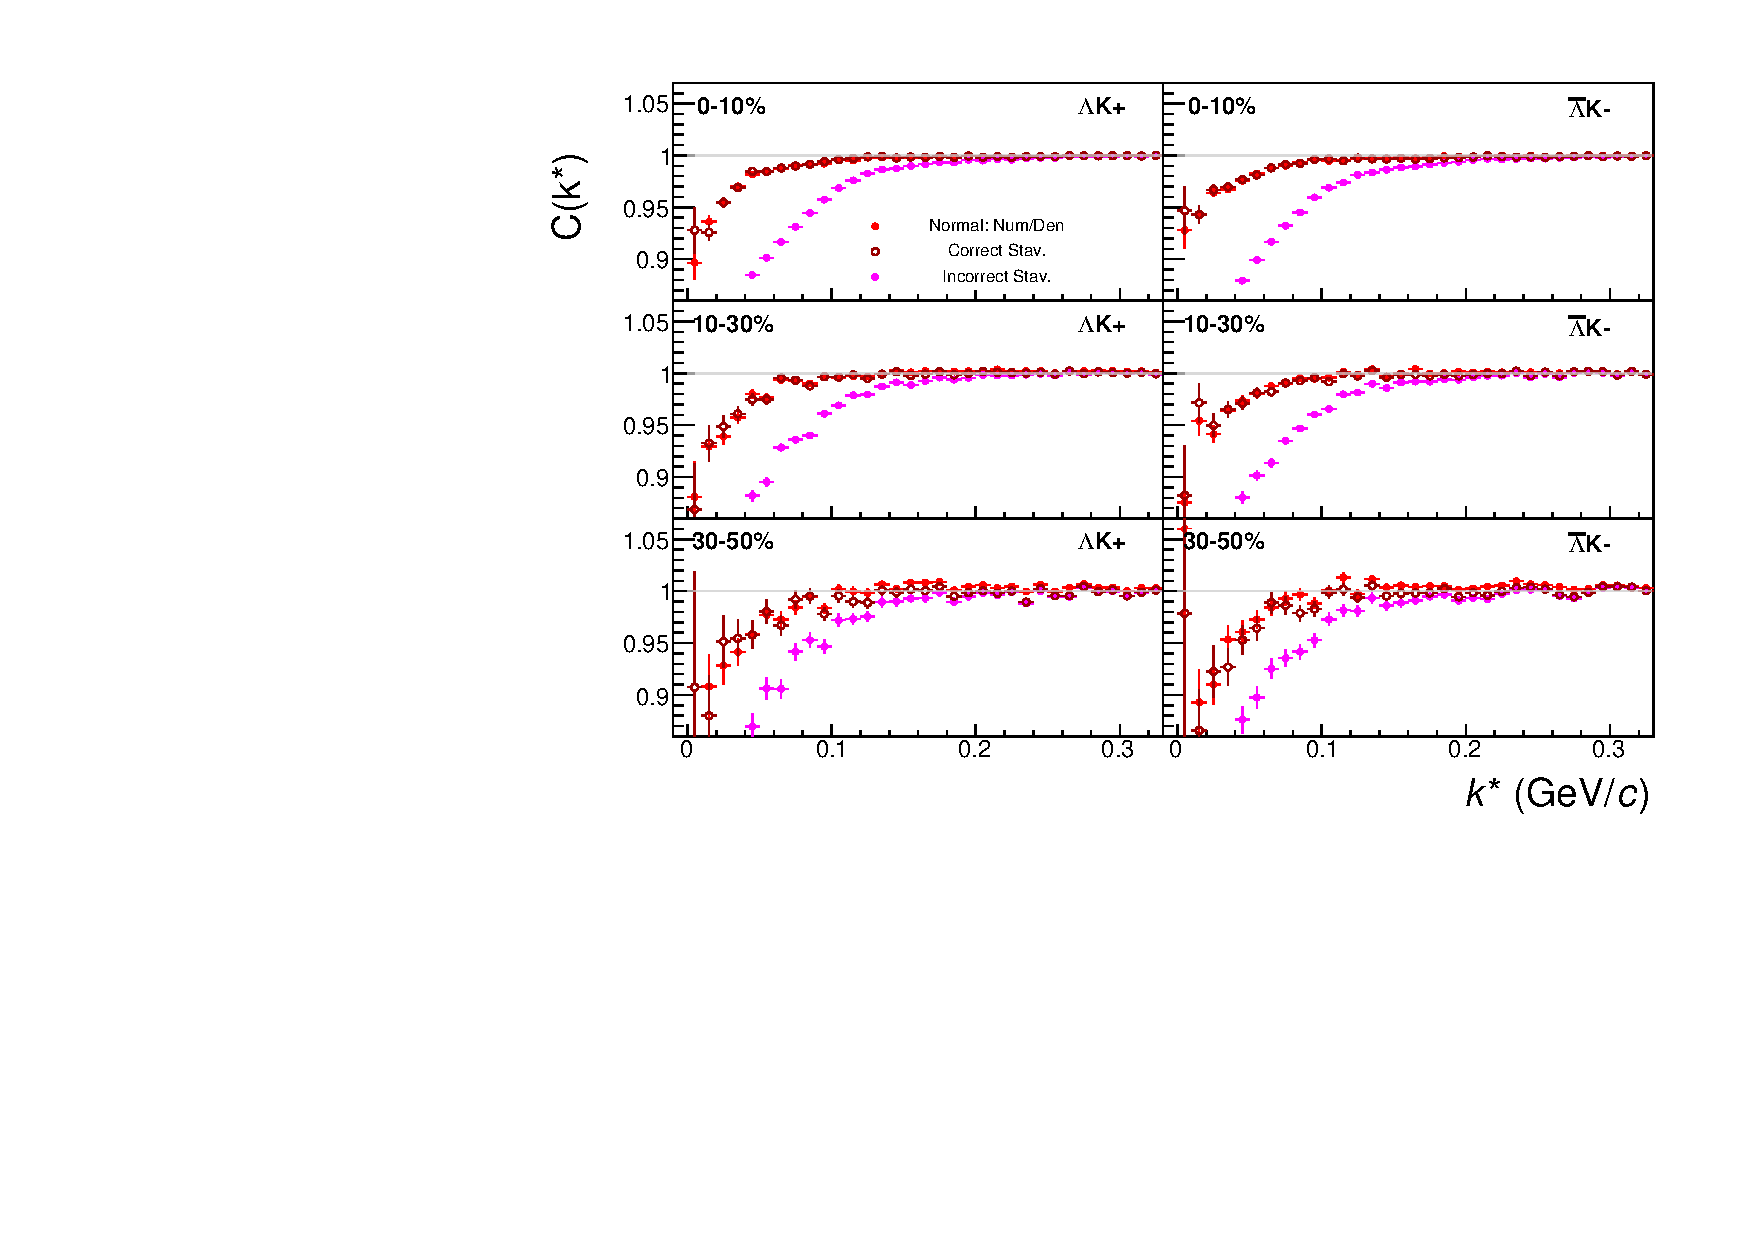
\includegraphics[width=0.49\textwidth]{4_CorrelationFunctions/Figures/AllThreeTogether/canKStarCfsZoomLamKchPwConj_20180505vs20180505StavCfvs20180416StavCf.pdf}}
  \\    
  
  %%----start of third subfigure---  
  \subfloat[\LamKchP (left) and \ALamKchM (right).  Incorrect Stavinsky shown as open symbols.]{
    \label{fig:AllStavCfs_CorrectAndIncorrect:c}
    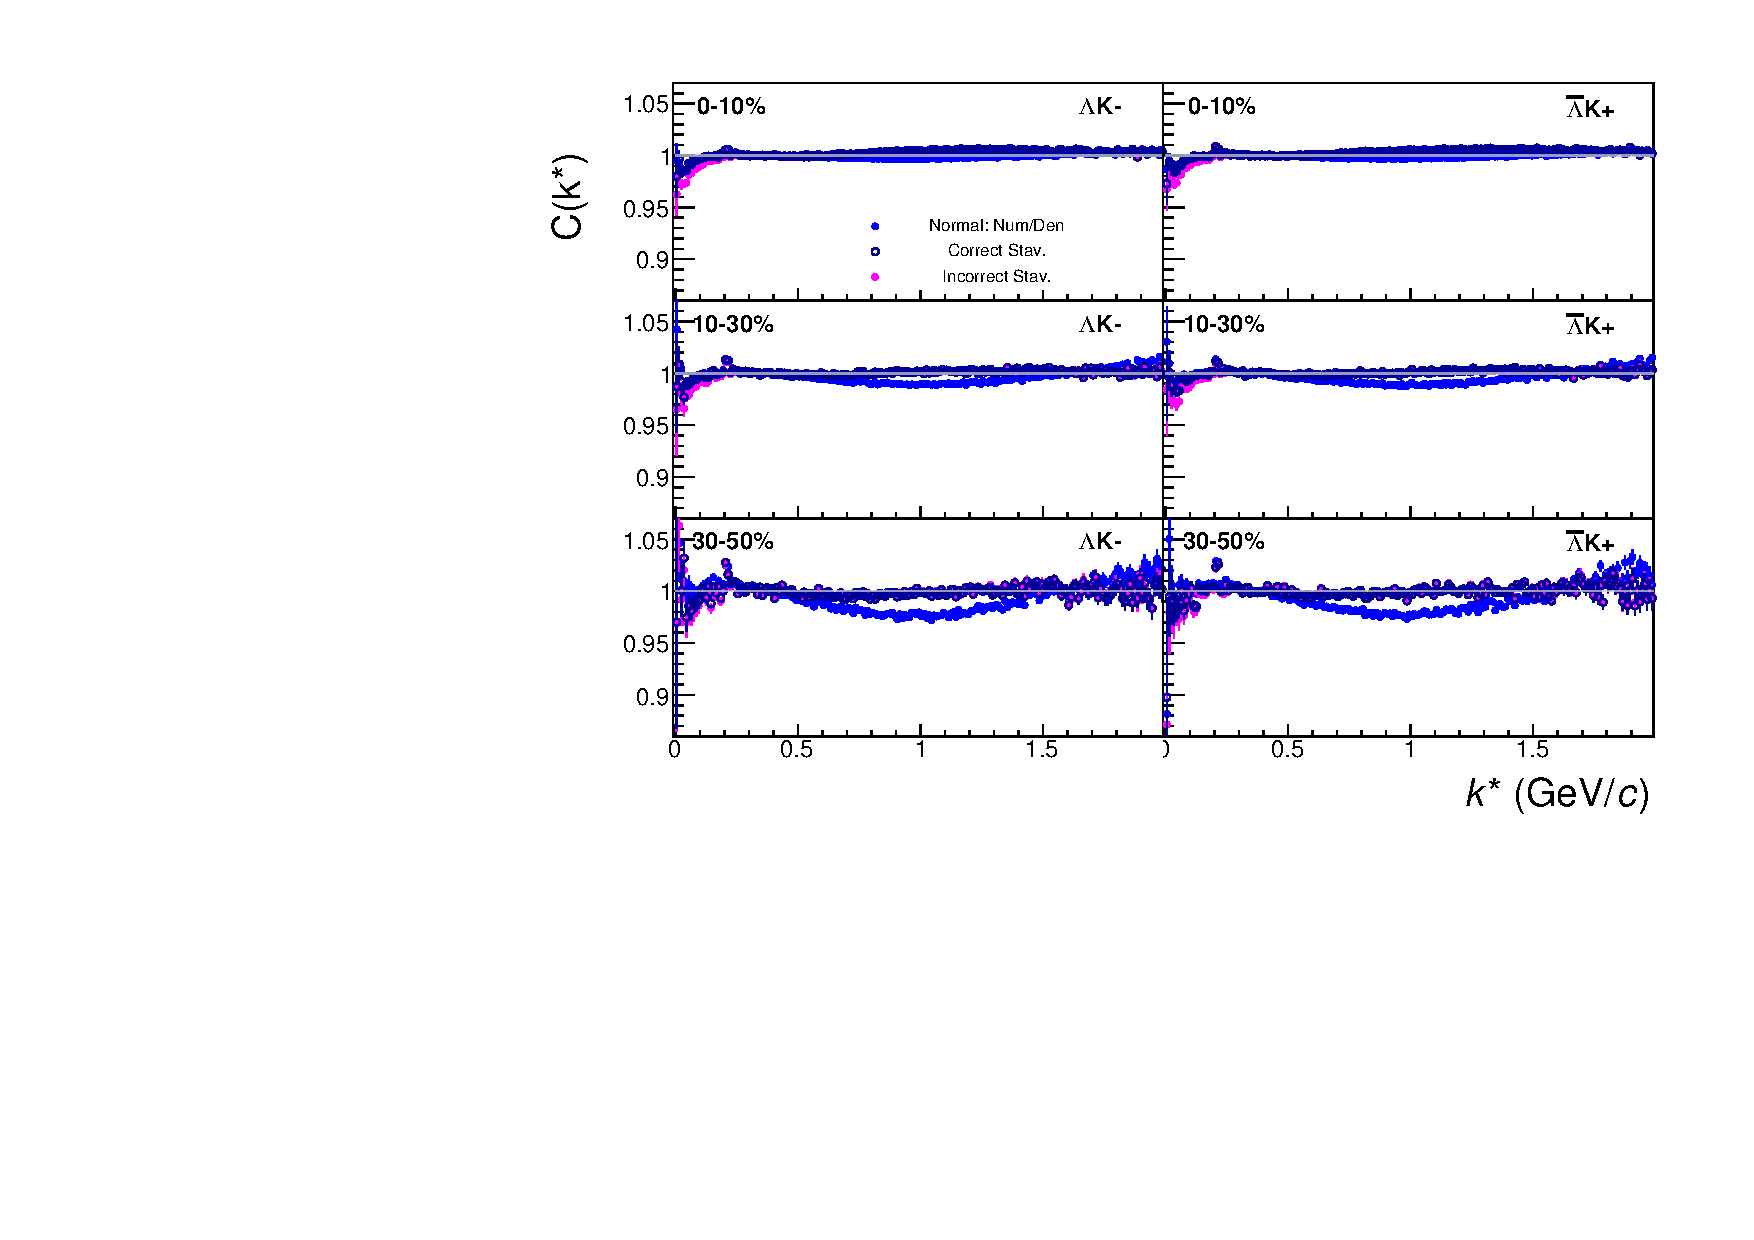
\includegraphics[width=0.49\textwidth]{4_CorrelationFunctions/Figures/AllThreeTogether/canKStarCfsLamKchMwConj_20180505vs20180505StavCfvs20180416StavCf.pdf}}
  %%----start of fourth subfigure---
  \subfloat[\LamKchM (left) and \ALamKchP (right).  Incorrect Stavinsky shown as open symbols.]{
    \label{fig:AllStavCfs_CorrectAndIncorrect:d}
    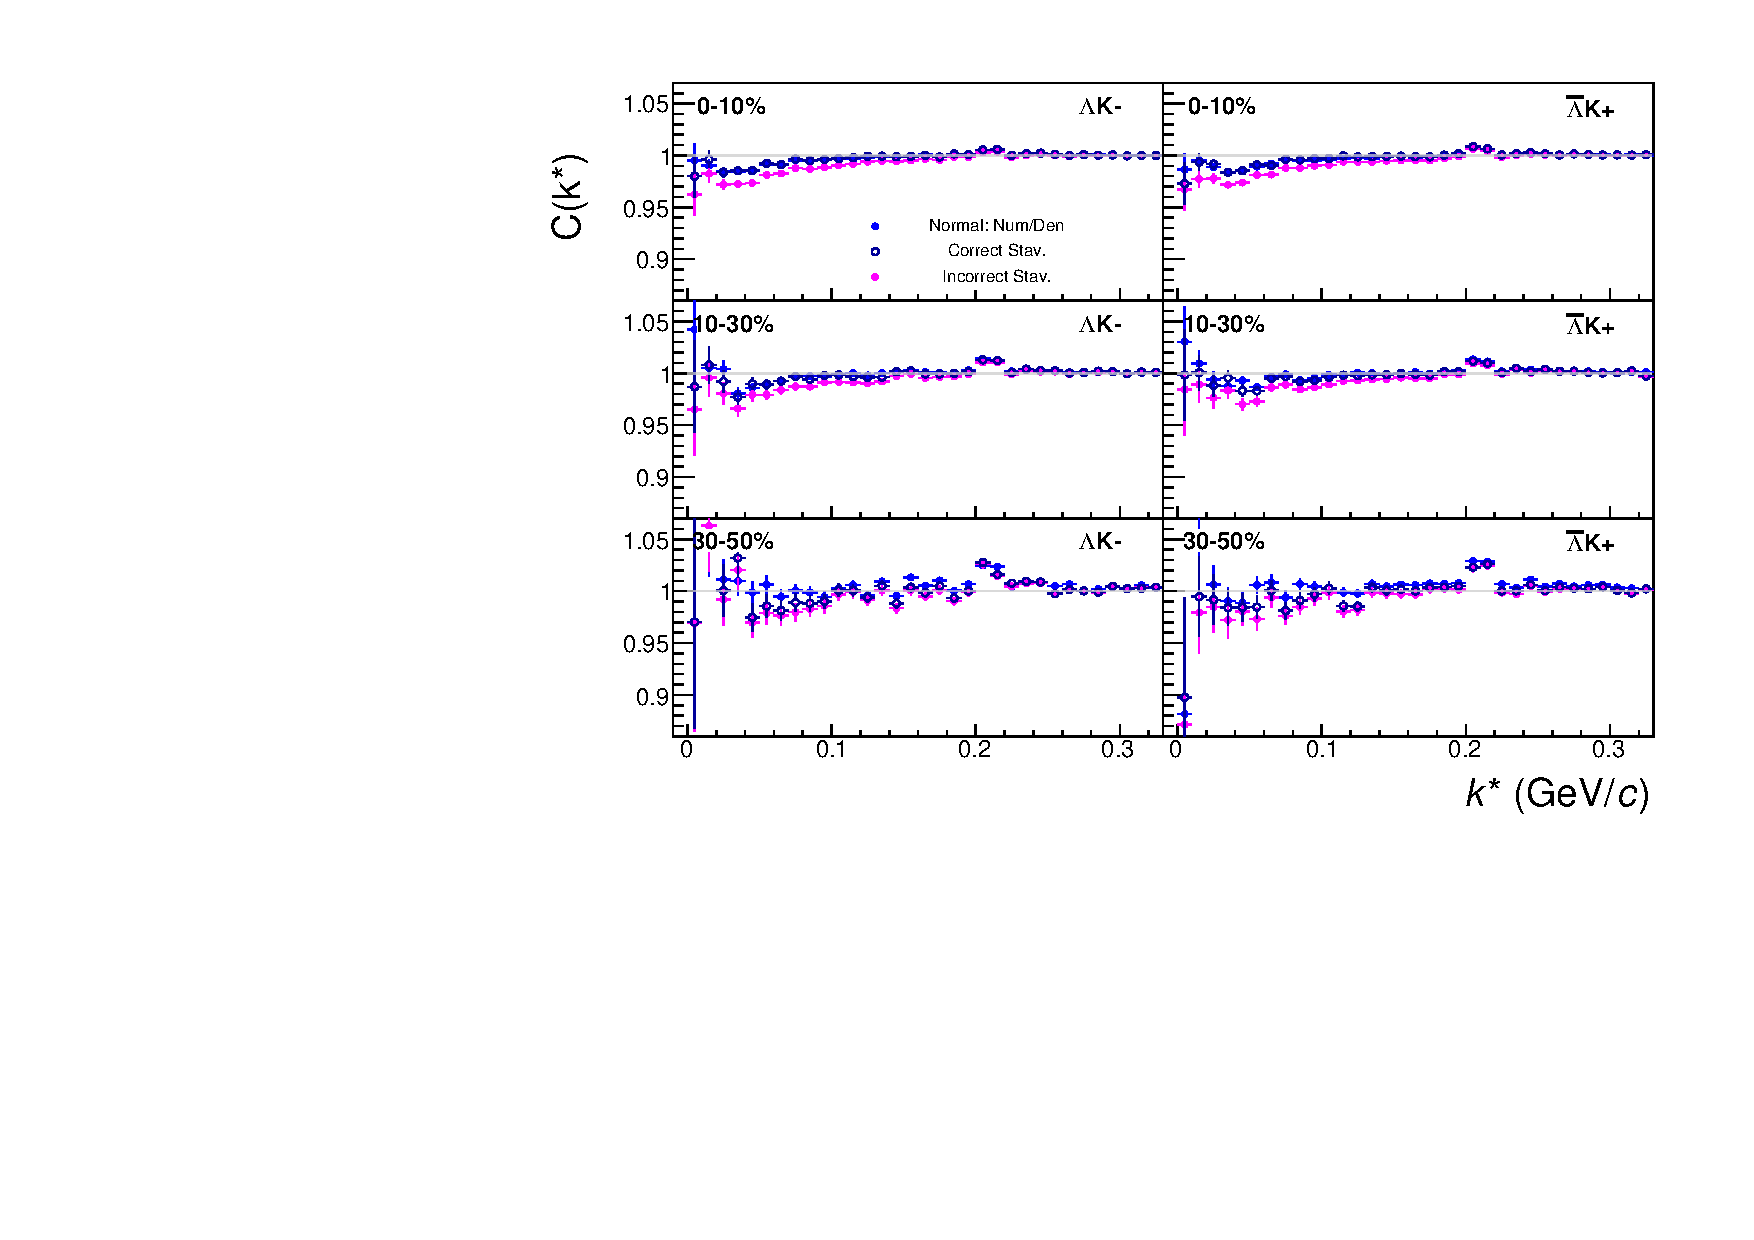
\includegraphics[width=0.49\textwidth]{4_CorrelationFunctions/Figures/AllThreeTogether/canKStarCfsZoomLamKchMwConj_20180505vs20180505StavCfvs20180416StavCf.pdf}}
  \\    
    
  %%----start of fifth subfigure---  
  \subfloat[\LamKchP (left) and \ALamKchM (right).  Incorrect Stavinsky shown as open symbols.]{
    \label{fig:AllStavCfs_CorrectAndIncorrect:e}
    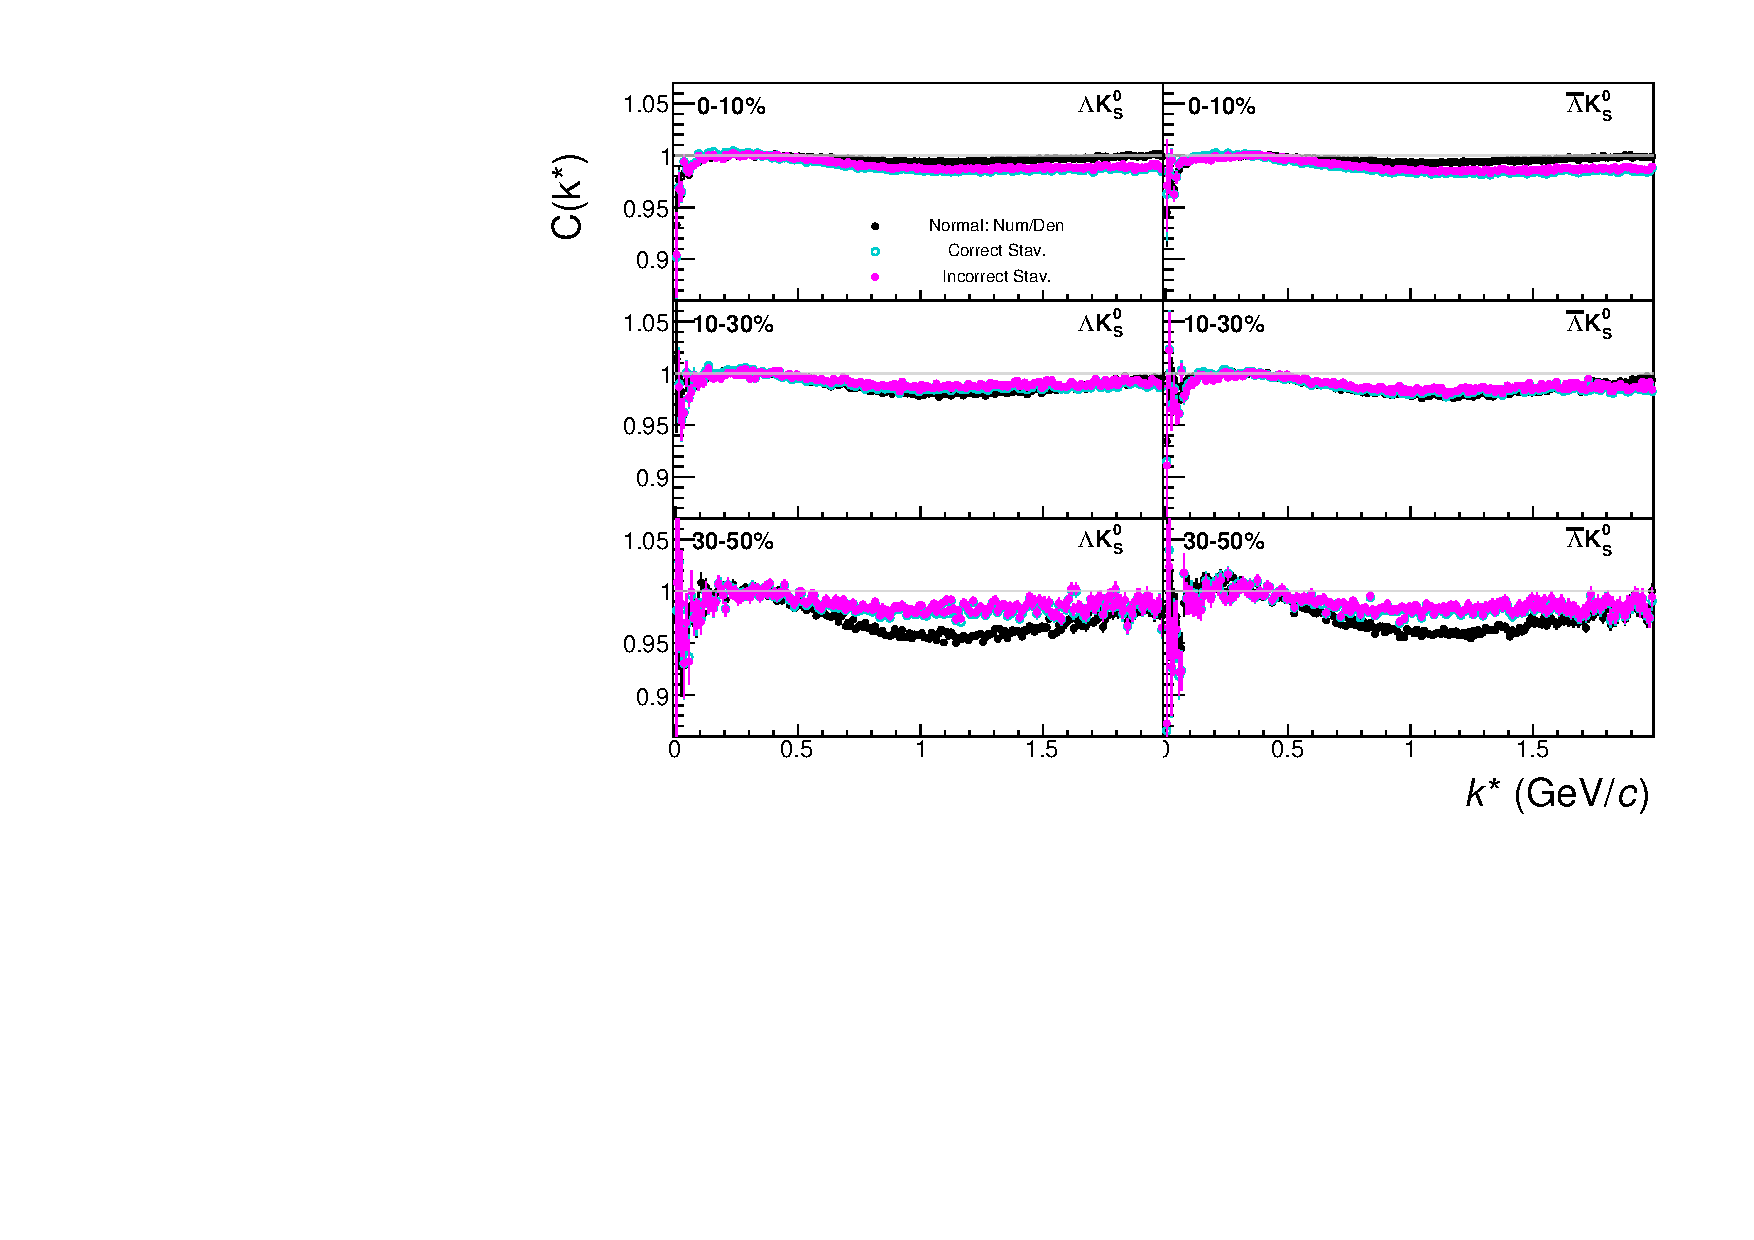
\includegraphics[width=0.49\textwidth]{4_CorrelationFunctions/Figures/AllThreeTogether/canKStarCfsLamK0wConj_20180505vs20180505StavCfvs20180416StavCf}}
  %%----start of sixth subfigure---
  \subfloat[\LamKchM (left) and \ALamKchP (right).  Incorrect Stavinsky shown as open symbols.]{
    \label{fig:AllStavCfs_CorrectAndIncorrect:f}
    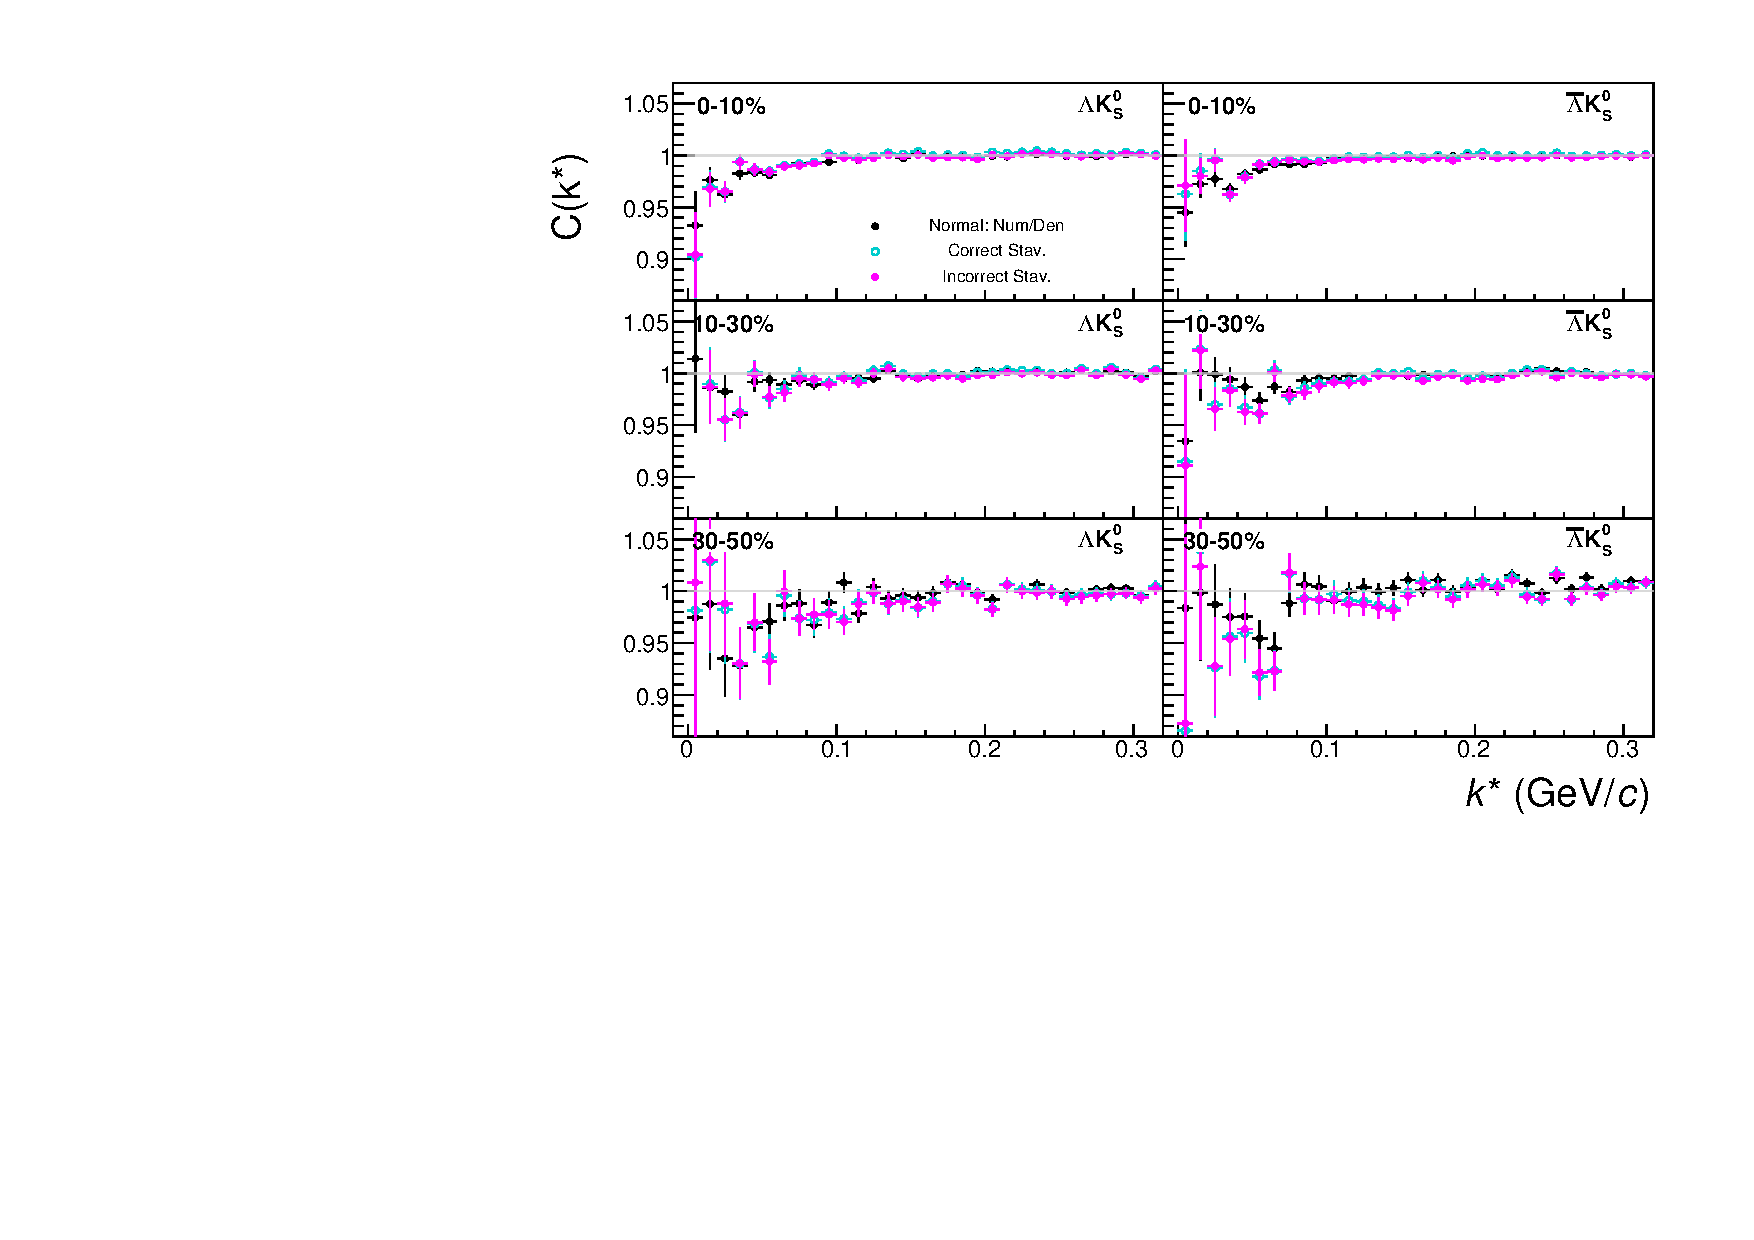
\includegraphics[width=0.49\textwidth]{4_CorrelationFunctions/Figures/AllThreeTogether/canKStarCfsZoomLamK0wConj_20180505vs20180505StavCfvs20180416StavCf}}
  \\         
    
  %%----overall caption----
  \caption[\LamK Stavinsky Correlation Functions (Correct and Incorrect)]{\LamK and \ALamAK correlation functions built using the Stavinsky method for 0-10\%, 10-30\%, and 30-50\% centralities.  The closed, (red, blue, black) symbols represent correlation functions formed using the normal method with mixed-event background pairs.  The open, cyan symbols represent correlation functions formed using the correct Stavinsky method.  The closed, magenta symbols represent correlation functions formed using the incorrect Stavinsky method.  In the incorrect method, the pseudo-pairs (same-event pairs with one particle rotated by 180$^\circ$ in the transverse plane) are not run through the pair cuts used in the analysis.  Figures in the right column are zoomed-in versions of figures in the left column.}
  \label{fig:AllStavCfs_CorrectAndIncorrect}
\end{figure}







\end{document}